\chapter{Methodology and Design}
This chapter will describe the methodology used in the project. Firstly, it gives a general description of the system and how the components relate to each other and where they are on the system. This broad overview is to create a point of reference so that in later sections the specific details of the system can be discussed without spending too much time on the broader aspects. A brief discussion on the software enviroment is also included to provided a justification for the use of the chosen enviroment. Finally, the chapter will go into the design of the system. The design will discuss the objectives and requirements and then move onto the specifics of the hardware, electronics, software and the control system. The focus of this project is the control system and so the hardware discussion will focus on how it is relevant and how it is integrated with the system. The electronics form integral parts to the control system and so they are discussed in further detail and finally the software and control system are the focus of the project and will be described in full.\par
\begin{figure}[hb]
	\begin{center}
		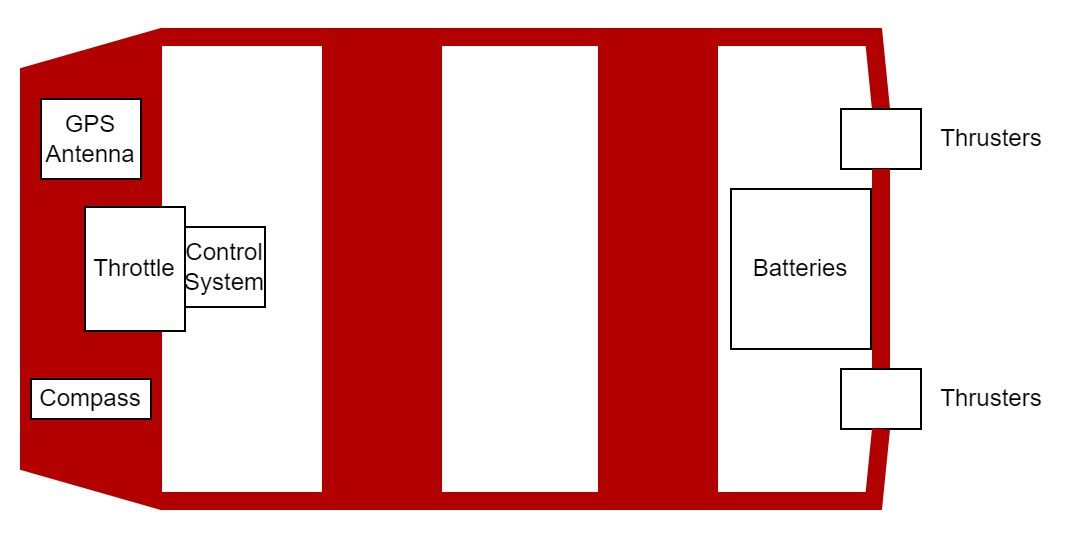
\includegraphics[width = 0.7\linewidth]{figures/BoatLayout.jpg}
		\caption{Broader System Diagram}
		\label{fig:3:boatDiag}
	\end{center}
\end{figure}
\section{System Description}
This section will give a broad overview of the system as a whole and  provide a reference of how the individual elements fit together both in the broader system and the narrower control system. The broader system is shown in Figure \ref{fig:3:boatDiag} and shows the vessel and the positions of the thrusters, batteries, control system throttle and mounting of the GPS antenna and compass. The control system refers to the 'motherboard', a PCB containing the microcontroller and other electronics including the GPS, SD module, logic level converter and the control box of switches and display LEDs. The wiring diagram of Figure \ref{fig:3:wiring} shows the PCB as a grey dotted line. The control box is shown outside of the PCB as it has its own housing but is affixed to the control system housing and is therefore considered part of the control system. Figure \ref{fig:3:wiring} also shows the wiring to the other elements that can be seen on the broader system diagram of Figure \ref{fig:3:boatDiag}. \par
\begin{figure}[ht]
	\begin{center}
		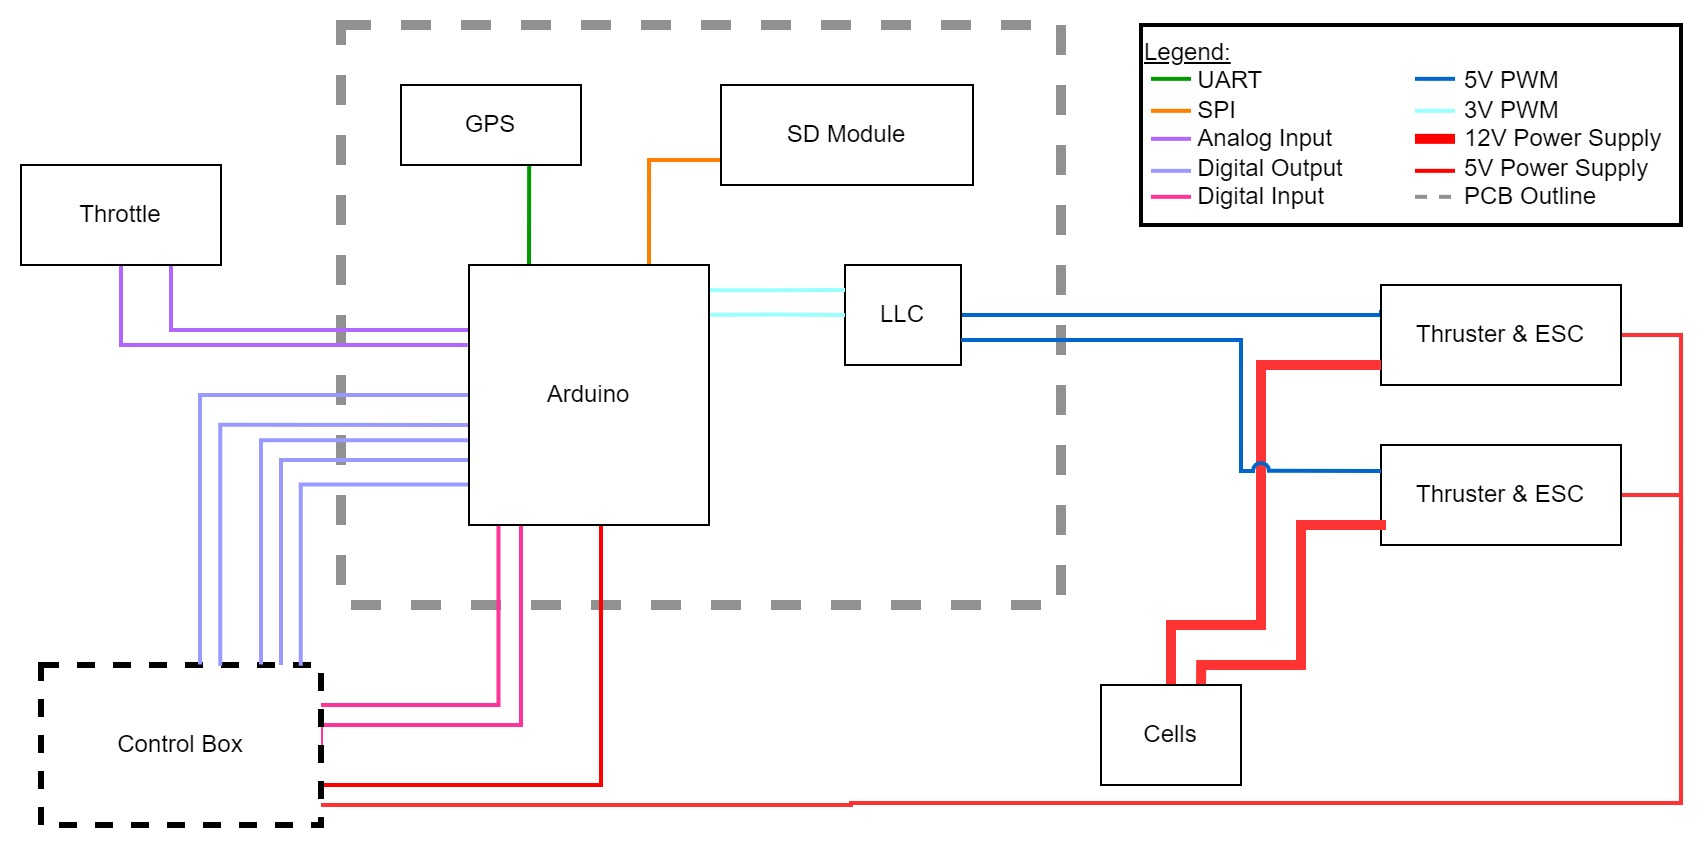
\includegraphics[width =\linewidth]{figures/Wiring diagram.jpg}
		\caption{Wiring Diagram for the System}
		\label{fig:3:wiring}
	\end{center}
\end{figure}

\section{Software Environment}
The microcontroller that was chosen for this project is an Arduino DUE. An Arduino microcontroller was chosen for the wide range of Arduino libraries available online, as well as several forums and code examples. Furthermore, the Arduino environment uses the C language which has been extensively covered through the course of the engineering degree. \par
\section{System Design}
	\subsection{Objective}
	The system needs to be designed to be deployed for long periods of time between services. The future addition of power regeneration such as solar or wind can be used to improve the deployable range and period of the vessel, but the energy storage must be designed to handle an extended period of 'dark time', any time when the power regeneration is negligible. \par
	The vessel must be autonomous and, having received a set of navigation points before deployment, navigate between these points until retrieval. Even under non ideal circumstances the vessel should be able to correct its course and continue to navigate to the set navigation points. \par
	This system is a proof of concept that is designed to be able to be sized up to a larger vessel. Therefore, the prototype vessel should be able to handle any conditions that could be encountered in testing and all electronics should be sufficiently sealed so that no damage is incurred. It is not expected that the prototype vessel would be able to handle rough and storm weather conditions.\par
	\subsection{Engineering Requirements}
	The prototype is a proof of concept that can be scaled up to a larger vessel and so a small vessel that can accommodate at least two people is required. This is preferred to a smaller vessel which cannot accommodate the weight of a person as the weight to power ratio of a small vessel could have an adverse effect on the steering capability of the vessel and therefore the control system.
	Furthermore, a working vessel is going to require a large battery bank and this is easily accommodated in a larger vessel. The energy source can then be scaled up by adding cells in both parallel and series to create the required power supply for the working vessel.\par
	The autonomous nature of the vessel means that an electronic control system is required to control the vessel. There are other elements that are required to make up the system, however these are not integral to the autonomous nature of the system but integral to the entire system. \par
	\subsection{Differential Steering} 
	Most ships and sea going vessels use a rudder or a directional thrusters to manoeuvre and this often simpler as it can be done with one thruster. However, in this project, the system has two thrusters and will make use of differential steering. Differential steering uses the two thrusters working at different thruster levels to steer the vessel. The outside thruster is at full power and the inside thruster is powered down and can even be put into reverse to manoeuvre the vessel. The most popular use of differential steering is in tracked vehicles such as military tanks. This project will use a system of progressive steering. Depending on how much the system needs to steer will determine how much thrust is given by the inside thruster. For example: for full steering the inside thruster will have \SI{100}{\percent} reverse thrust but for only a small steering correction the inside thruster could be powered down to \SI{80}{\percent}.
\begin{figure}
	\begin{center}
		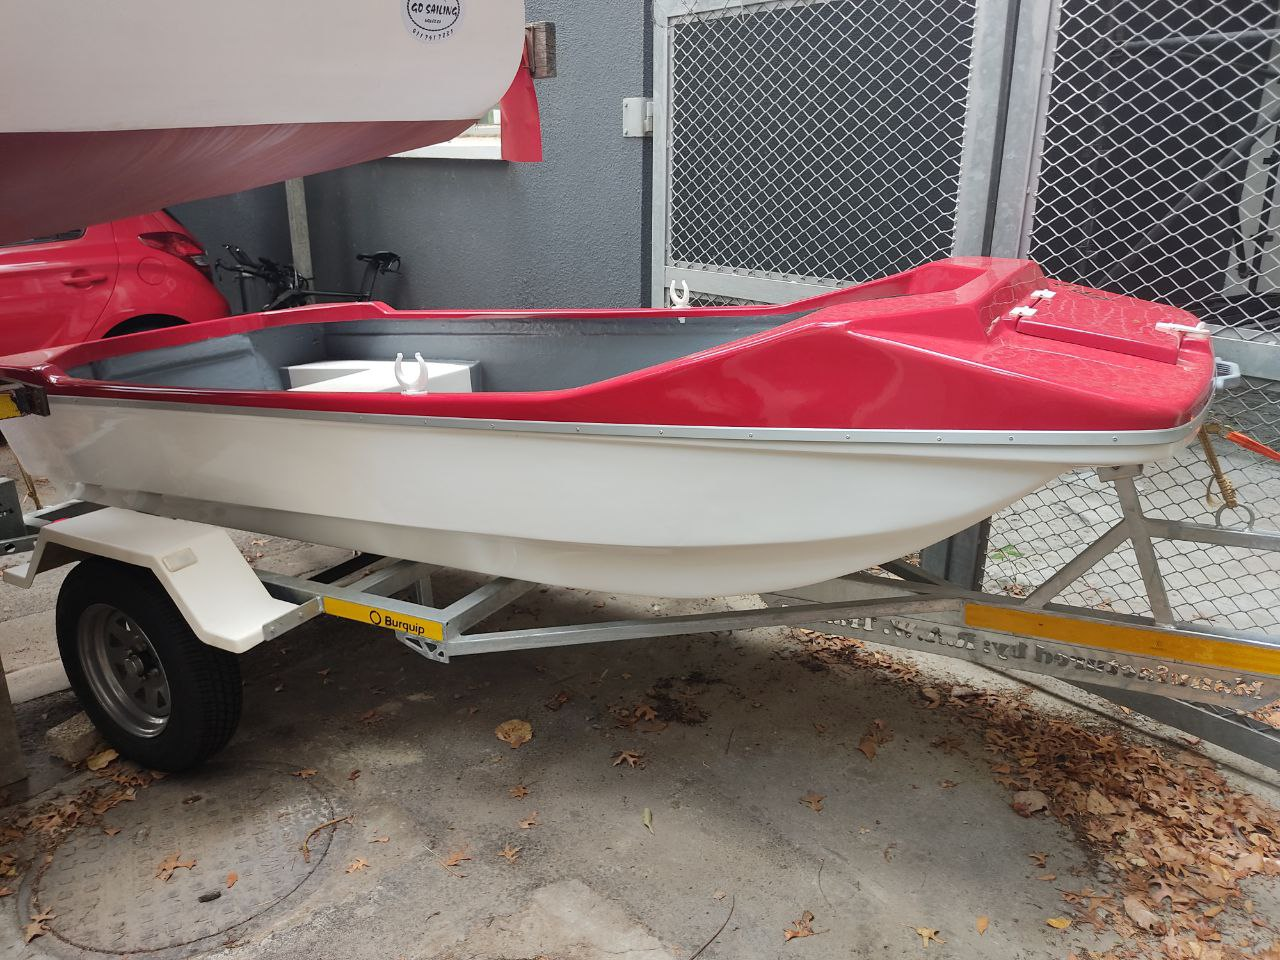
\includegraphics[width = 0.65\textwidth]{figures/spider3.jpg}
		\caption{The vessel, a Spider 3.}
		\label{fig:3:spider}
	\end{center}
\end{figure}
	\subsection{Hardware}\par
		\subsubsection{Vessel}
		The vessel is outside the scope of this project as it was acquired before the start of the project. The project was designed around the use of the vessel for testing only as in actual use a vessel would be used that could handle severe weather conditions and hold an array of sensory equipment. The vessel pictured in Figure \ref{fig:3:spider} is a Spider 3, a small single hulled fibreglass boat. The vessel measures \SI{1.3}{\meter} $\times$ \SI{3.2}{\meter} and is rated to carry four people and a 15 Hp traditional outboard motor.\par
		\subsubsection{Thrusters}
		The thrusters are electrical and a complete unit together with the ESC, and all the electronic interfacing to drive the thrusters is accomplished through it. The ESC is described later in the report. Therefore, the thrusters are considered general hardware and are there only as a means of testing the control system. They are outside the scope of the project as they were acquired prior to the start of the project, but are integral to the performance of the overall system.\par 
		The propulsion system consists of two electric thrusters mounted at the back of the vessel. These thrusters are each capable of producing up to \SI{18}{\kilogram} of thrust. An aluminium mount designed and manufactured by the Stellenbosch University Electrical Engineering workshop allows for the thrusters to be raised during the launching and retrieval of the boat to avoid fouling on the trailer. The mounts are removable and are removed for transport. Each thruster has an integrated ESC that regulates the power supplied to the electric motor and therefore the thrust provided.
		\subsubsection{Power Supply}
		The initial design was to use a bank of four Lithium Iron Phosphate (LiFePO) cells to form a \SI{12}{\volt} battery. This was also procured before the start of the project. However, upon testing, it was seen that \SI{12}{\volt} was not enough voltage to provide the thrusters with enough power to move the boat at a reasonable rate. Each cell has a voltage of \SI{3.3}{\volt} and a capacity of \SI{100}{\ampere\hour}. Therefore, the next course of action was to source more cells and increase the size of the battery. However, due to the high cost of these cells and a lack of suppliers this was not plausible. LiFePO cells are expensive because they are designed to have a deeper life cycle than standard lead acid cells. These cells in particular were also expensive due to their large capacity.\par 
		Therefore, the decision was made to change the power source to a battery consisting of two lead acid cells in order to test the control system. The lead acid cells were each \SI{12}{\volt} and had a capacity of \SI{50}{\ampere\hour}. A lead acid battery can generally be drained to about \SI{80}{\percent} capacity without doing much damage to the cell, a LiFePO cell has a deep cycle of about \SI{40}{\percent}-\SI{50}{\percent}. Therefore these cells would be used for short tests and recharged between tests. However, for a working system it would be recommended that a large LiFePO battery bank were used. 
		\begin{figure}[!ht]
			\begin{center}
				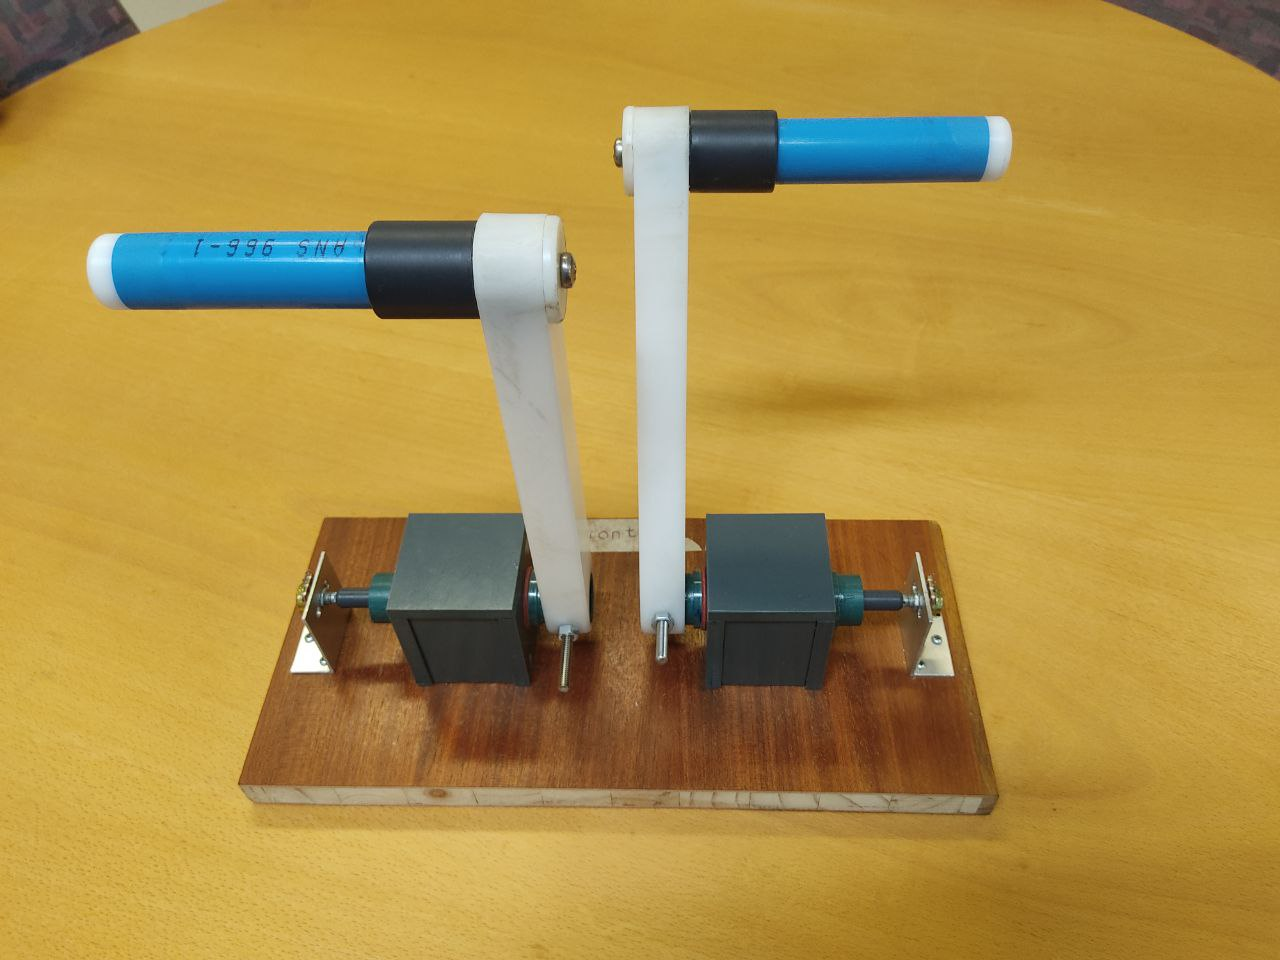
\includegraphics[width = 0.55\textwidth]{figures/throttle.jpg}
				\caption{Final throttle system with two potentiometers (POT) on either end.}
				\label{fig:3:throttle}
			\end{center}
		\end{figure}
		\subsubsection{Throttle}
		The initial concept was to purchase two throttles capable of moving independently from each other and two electronic throttle levers were purchased to be used. However, when these components arrived, they were much smaller than they had appeared and had a very small range of movement. An alternate solution was designed consisting of two throttle arms that could each turn a shaft. These shafts were then connected to a linear potentiometer which would provide the required analogue input from the throttle. The throttle is shown in Figure \ref{fig:3:throttle}. An initial concept design was given to the electrical engineering department who then refined and manufactured the design. 
		\par
	\subsection{Electronics}\par
		
		\subsubsection{Arduino Due}\par
		\begin{figure}[!ht]
			\begin{center}
				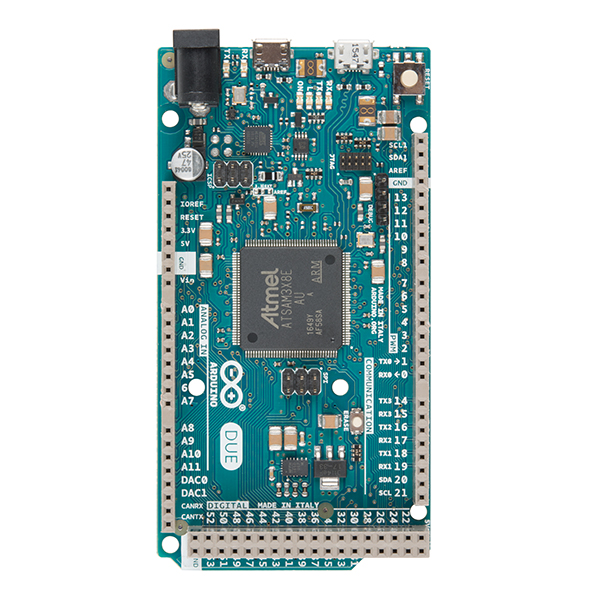
\includegraphics[width = 0.48\textwidth]{figures/DUE.jpg}
				\caption{The microcontroller used: an Arduino DUE}
				\label{fig:3:due}
			\end{center}
		\end{figure}
		The microcontroller was selected by considering the initial design and possible peripherals that would be used in the system. The minimum requirements for the microcontroller to be used are as follows, with regard to the peripherals of the GPS, SD card modules, the ESC and POTs as well as several inputs and outputs:
		\begin{enumerate}
			\item 2 PWM pins.
			\item Voltage regulators of \SI{3}{\volt} and \SI{5}{\volt}.
			\item 5 digital IO pins.
			\item 4 analogue input pins.
			\item 1 SPI connection.
			\item 1 UART connection.
			\item 1 I\textsuperscript{2}C connection.
			\item \SI{256}{\kilo\byte} programmable flash memory.		
		\end{enumerate}
		Based on these requirements, the Arduino Uno was considered. It is the standard Arduino board used in projects and meets most of the minimum requirements for the project.  However, the Arduino Uno has only one UART connection and does not allow for any possible design alterations that might need a second UART connection. Finally, the Arduino only has \SI{32}{\kilo\byte} of programmable flash memory which does not meet the requirements.\par 
		The next consideration was the Arduino DUE, shown in Figure \ref{fig:3:due} This has 4 UART connections, plenty of digital IO pins and several analogue inputs. This offers a range of versatility to any design progression or alterations that might occur. Furthermore, the DUE has \SI{512}{\kilo\byte} of programmable flash memory which is double that of the minimum requirement. The one flaw with the Arduino DUE is that its IO pins operate at \SI{3.3}{\volt} as opposed to the generally standard \SI{5}{\volt}. However, this was easily overcome by implementing a logic level converter to shift the required signals to \SI{5}{\volt} while keeping the signals' shape. Keeping the signals' shape is particularly important for the PWM signal controlling the ESCs. The final microcontroller selected was the Arduino DUE. \cite{Corporation2015}
		\subsubsection{SD Card Module}
		The SD card is used as an external storage device. Data can then be written to the SD card during operation and the data can be downloaded for analysis. The SD card module is a standard SD card module that is attached to the microcontroller as shown in the wiring diagram Figure \ref{fig:3:wiring}. The SD card uses SPI communication and there are built-in libraries that are available for use. \cite{Association2017}
		\subsubsection{GPS Module}
		Initially a PmodGPS was used as the GPS module. However the PmodGPS has a built-in antenna and there were signal strength issues. The GPS was slow at acquiring a GPS fix when the control box was closed. Therefore, an alternate GPS module with an external antenna was sourced. The antenna can be fed out of the control box and positioned where a strong signal can be received. Both GPS modules use UART to communicate the data to the microcontroller. The GPS modules send a string of characters along the UART connection, and the microcontroller must then decode the characters. The GPS module transmits the current longitude, latitude, date and time and speed of the vessel to the microcontroller. The UART is set-up to use a baud rate of 9600, 8 data bits, no parity and 1 stop bit. It has two connectors J1, which has 6 pins and J2 which has 2 pins. J1 is used to power the GPS module as well as connect to the MCU using UART communication. \cite{Robot}
		\subsubsection{Compass}
		The digital compass used can be more accurately referred to as a magnetometer. The module used in this project, a  Pololu LSM303 shown in Figure \ref{fig:3:compass}, is a combination magnetometer and accelerometer, however only the magnetometer is used. Pololu has a range of Arduino libraries including a compass library for the LSM303 which is used to calibrate the module and to get an accurate compass bearing. \cite{STMicroelectronics2015}
		\begin{figure}[!hb]
			\begin{center}
				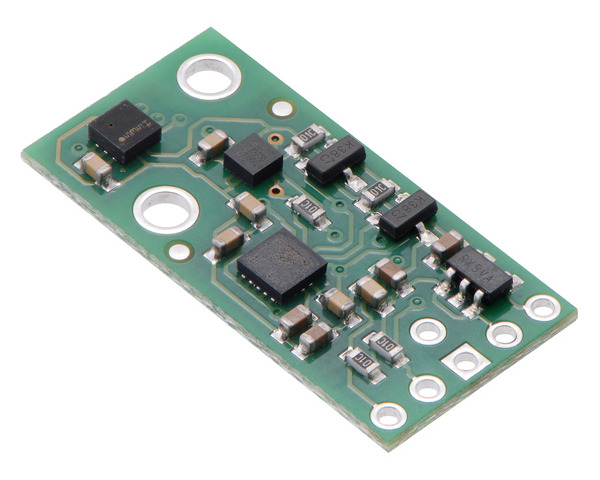
\includegraphics[width = 0.16\textwidth]{figures/compass.jpg}
				\caption{Pololu LSM303 AltIMU module.}
				\label{fig:3:compass}
			\end{center}
		\end{figure}
		\subsubsection{ESC}
		There are two ESCs, one for each thruster and are submersible. The ESC has two inputs, the control input, and the power input. Th power input can range between DC \SI{12}{\volt} and DC \SI{50}{\volt} and a maximum constant current of \SI{100}{\ampere} and in this project the input is \SI{24}{\volt} supplied by the battery cells. The control input is a \SI{5}{\volt} signal that is used to control the speed of the thrusters. This is a PWM signal whose duty cycle determines the thrusters RPM and therefore the speed and direction of the vessel. 
		\subsubsection{POT}
			\begin{table}[ht]
			\begin{center}
				\caption{The digital values of the ADC used to calibrate the physical limits and neutral range of the throttle potentiometers.}
				\label{tab:3:POT}
				\begin{tabular}{|l|c|c|}
					\hline		
					\textbf{Throttle Position} & \textbf{Left POT} & \textbf{Right POT} \\
					\hline
					Full Forward & 655 & 720\\
					\hline
					\multirow{2}{*}{Neutral} &440 &505 \\
					&485 &572  \\
					\hline
					Full Reverse & 285 & 352 \\
					\hline
				\end{tabular}
			\end{center}
		\end{table}
		The POT is a standard \SI{10}{\kilo\ohm} potentiometer that has three pins as shown in Figure \ref{fig:3:POTdraw}: high voltage, ground, and output. The high voltage and ground are connected to the outer pins on the POT and the output is connected to the centre pin. As the shaft of the potentiometer is rotated, the resistance varies from almost no resistance to the full \SI{10}{\kilo\ohm} which causes the voltage to vary from input, \SI{3.3}{\volt} to an almost ground voltage, ~\SI{0.1}{\volt}.  \par
		\vspace{0.4cm}
		\begin{figure}[hb]
			\begin{center}
				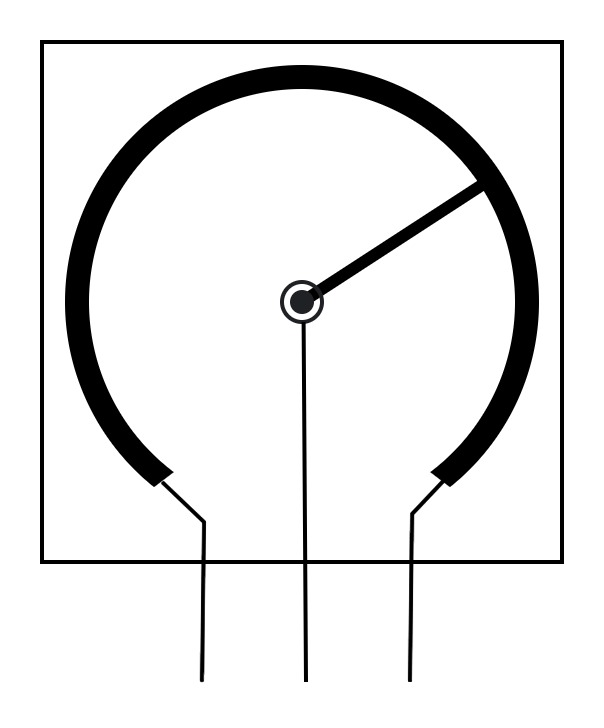
\includegraphics[width = 0.25\textwidth]{figures/POT.jpg}
				\caption{Simple illustration of a linear potentiometer}
				\label{fig:3:POTdraw}
			\end{center}
		\end{figure}
		The output is connected to analogue input pins on the microcontroller which uses an ADC, with a 10 bit resolution, to convert the signal to a value between 0 and 1024. However, the potentiometer has a \SI{300}{\degree} range of motion but the throttle has approximately \SI{150}{\degree} range of motion. The software can  correct for the difference by determining the total maximum and minimum range of motion of both throttle levers while in operation. The forward range is set between an offset middle point and maximum range for each device. Similarly, the reverse range is set between the offset middle point and the minimum range for each device.  This offers a neutral range buffer to make the throttle easier to use i.e. the controller can be placed in the neutral position by returning the lever to the general neutral position. The extents of the measured forward and reverse ranges are listed in Table \ref{tab:3:POT}.
	\subsubsection{Switches and LEDs}
	\begin{figure}
		\begin{center}
			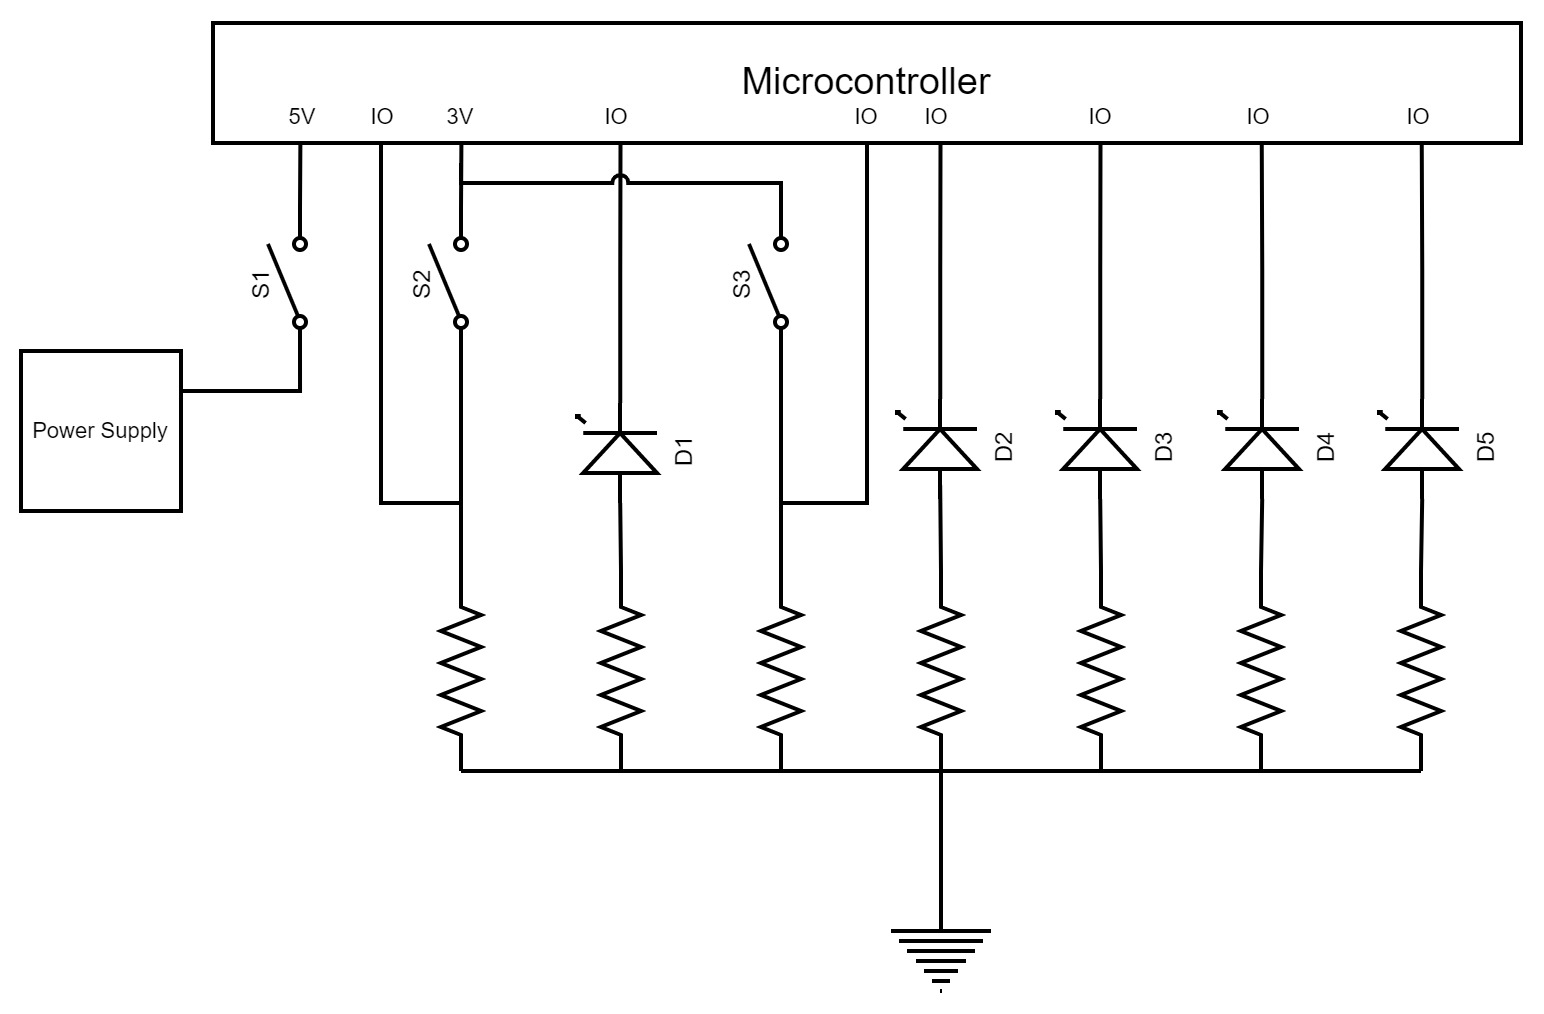
\includegraphics[width=0.65\linewidth]{figures/BoxCircuit}
			\caption{The wiring circuit inside of the control box.}
			\label{fig:3:controlCircuit}
		\end{center}
	\end{figure}
	The control box shown in Figure \ref{fig:3:controlBox} consists of 3 switches and 5 state display LEDs. Two of the switches are configured using pull down resistor configuration with the output of the pull down circuit connected to a digital input on the microcontroller. The LEDs all use simple LED circuits driven by the digital outputs of the microcontroller. The final switch, the power switch, is wired to cut-off the \SI{5}{\volt} power supply to the microcontroller. The control box circuit is shown in Figure \ref{fig:3:controlCircuit} and can also been seen in the overall wiring diagram of the system in Figure \ref{fig:3:wiring}. A description of each switch and LED is given in Table \ref{tab:3:controlBx}.
	\begin{figure}[hb]
		\begin{center}
			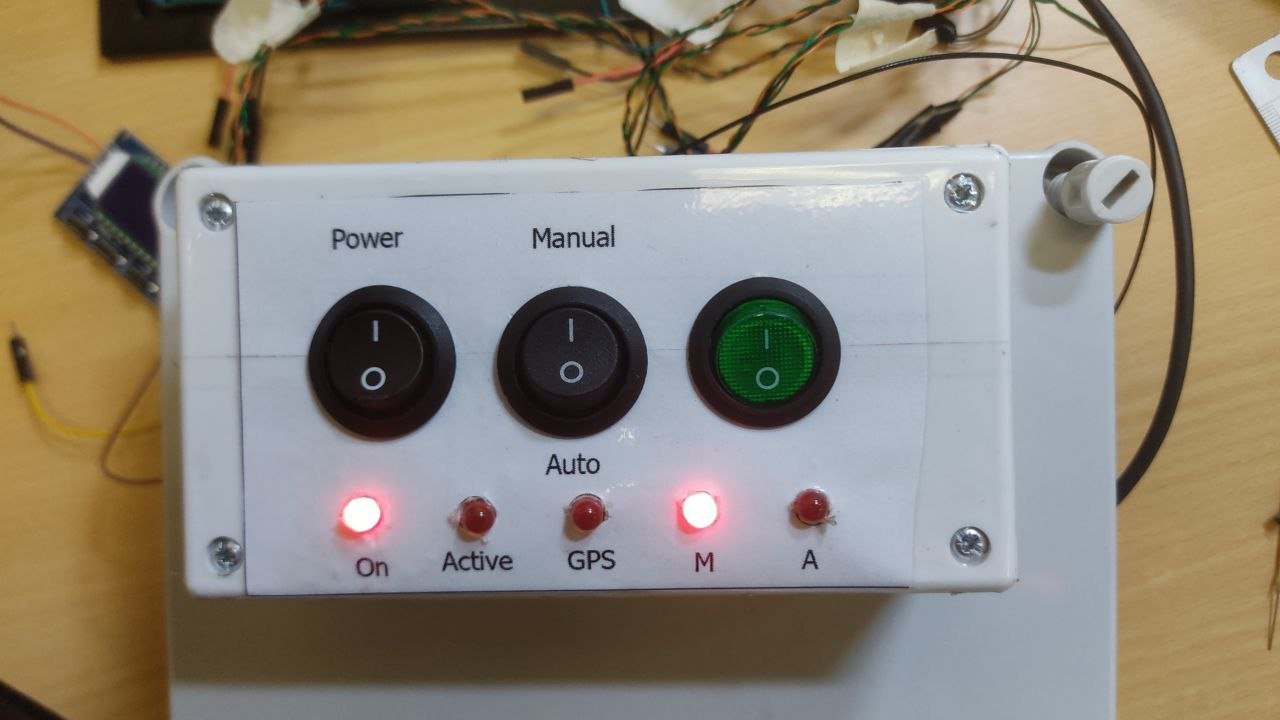
\includegraphics[width = 0.85\textwidth]{figures/controlBox.jpg}
			\caption{The control box with its 3 switches and 4 LEDs.}
			\label{fig:3:controlBox}
		\end{center}
	\end{figure}
	\begin{table}[ht]
	\begin{center}
		\caption{Description of the switches and LEDs on the control box.}
		\label{tab:3:controlBx}
		\begin{tabular}{|p{0.2\linewidth} | p{0.15\linewidth}|p{0.65\linewidth}|}
			\hline
			Component & Designation & Description \\
			\hline
			Power Switch & S1 & This switch is used to cutoff the power being supplied to the microcontroller. \\
			\hline
			Navigation Mode Switch & S2 & This switch allows the user to quickly switch between the manual navigation mode and the autonomous navigation mode. \\
			\hline
			Calibration Switch & S3 & This switch is used to put the system into compass calibration mode. \\
			\hline
			On LED & D1 & This LED indicates that the microcontroller is powered on. \\
			\hline
			Active LED & D2 & This LED blinks on and off during the operation of the program and indicates that the program is alive and active and there has not been a crash in the program. \\
			\hline
			GPS LED & D3 & This LED is turned on when GPS has a valid connection. \\
			\hline 
			M LED & D4 & This LED indicates that the system is in manual control mode. \\
			\hline
			A LED & D5 &  This LED indicates that the system is in autonomous navigation mode. \\
			\hline
		\end{tabular}
	\end{center}
\end{table}
	\subsection{Software}
	\subsubsection{PWM Signal}
	\begin{figure}[!hb]
		\begin{center}
			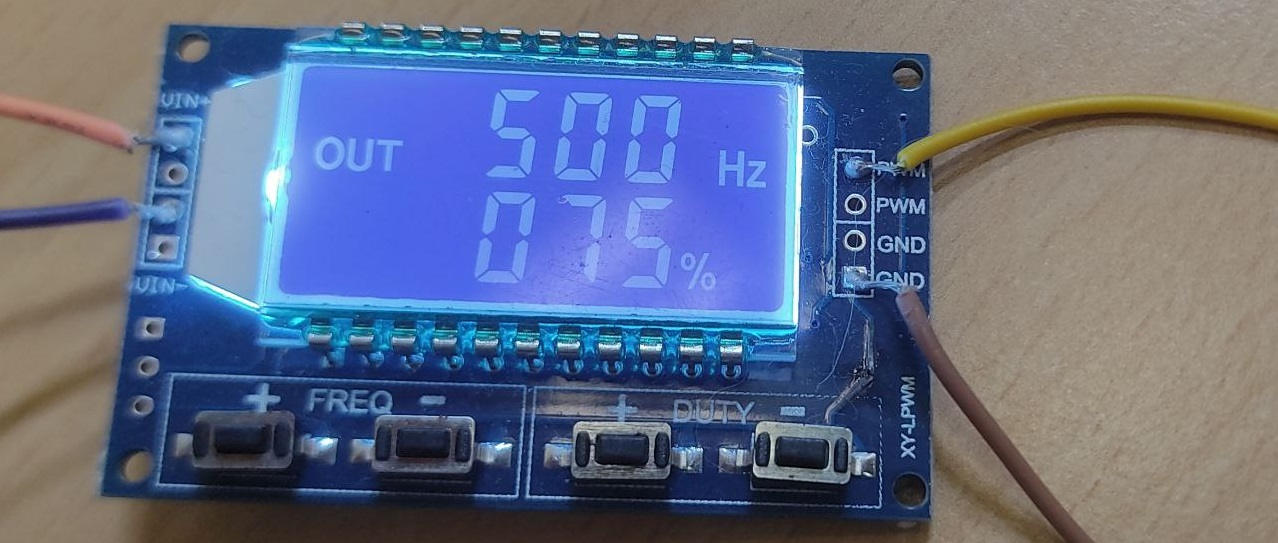
\includegraphics[width=0.31\linewidth]{figures/pwmGen.jpg}
			\caption{The PWM signal generator used to ensure the ESC was working.}
			\label{fig:3:PWMgen}
		\end{center}
	\end{figure}
	\begin{table}[!ht]
		\begin{center}
			\caption{ESC boundaries and PWM duty cycle at various frequencies.}
			\label{tab:3:PWM}
			\begin{tabular}{|l|c|c|c|c|}
				\hline
				\multirow{2}{*}{Position} & \multirow{2}{*}{Time (\SI{}{\micro\second})} & \multicolumn{3}{c|}{Duty Cycle @}\\
				%\hline 
				& & \multicolumn{1}{c}{\SI{50}{\hertz}} & \multicolumn{1}{c}{\SI{60}{\hertz}} & \multicolumn{1}{c|}{\SI{500}{\hertz}}\\
				\hline
				Full Forward & 2000 & \SI{10}{\percent} & \SI{12}{\percent} & \SI{100}{\percent}  \\
				\hline
				Neutral & 1500 & \SI{7.5}{\percent} & \SI{9}{\percent} & \SI{75}{\percent}  \\
				\hline
				Full Reverse & 1000 & \SI{5}{\percent} & \SI{6}{\percent} & \SI{50}{\percent}  \\
				\hline
			\end{tabular}
		\end{center}
	\end{table}
	The thrusters are each controlled by a \SI{5}{\volt} PWM signal. There is limited information on the datasheet for the ESC. The signal boundaries, full forward, full reverse and neutral positions are described in the unconventional terms of the time that the signal is high. The values are shown in Table \ref{tab:3:PWM}. Initially it was thought that the ESC operated at \SI{50}{\hertz}, however there was no response from the thruster at any duty cycle when using this frequency.A PWM signal generator IC, shown in Figure \ref{fig:3:PWMgen}, was connected to ESC to ensure  the correct PWM signal was being sent through and to quickly vary both the frequency and the duty cycle.  Trial and error later determined that the ESC began responding to a signal above \SI{60}{\hertz}. It was then decided to push the frequency up to the maximum of \SI{500}{\hertz} as this offers the finest control because it has the maximum allowable duty cycle difference between the signal boundaries.\par
	\vspace{0.4cm}
	The Arduino libraries contain a function, \textit{analogueWrite(value, pin)}, which takes the duty cycle and the output pin as parameters. This will output a PWM wave of the given duty cycle on the given pin. However, the default frequency of the Arduino DUE PWM pins is \SI{1000}{\hertz}. Therefore, the frequency had to be manually changed by changing the timer settings driving the PWM signal.\par
	\vspace{0.4cm}
	The information needed to change the timer settings is available in the Arduino Datasheet. The process to configure the PWM outputs is as follows. First, the peripheral clocks for timer channels 6 and 7 were enabled. Secondly, the pins' input-output controller on peripheral A needed to be disabled and the pins switched to peripheral B. Then came the configuration of the timer itself. The channel mode was set to waveform mode using clock 1 with the timer counter being incremented on the rising edge. Furthermore, the waveform was set to UP mode (signal is set high) being triggered when the counter reached the register C (RC) value and the signal being cleared when the counter reached the register A (RA) value. Once the timer is configured, values can be assigned to the RA and RC values, and the interrupt set to trigger when the counter reaches RC. Finally, an interrupt handler needs to be added to read the status register, since the flags in the status register are automatically reset when it is read at the end of every period.\par
	\vspace{0.4cm}
	The signal is cleared when the counter reaches RA and set high when the counter reaches RC. Therefore, RC can be equated to the period of the signal and RA to the time when the signal is high. Since the clock is set to clock 1 which is the MCU clock (MCK) divided by 2, and by using the above comparison, the RA and RC can then be expressed in terms of MCK, frequency and duty cycle, as shown in Equations \ref{eq:3:RC} and \ref{eq:3:RC}. RC is kept constant throughout while RA is changed to adjust the duty cycle of the PWM signal sent to the ESC, thereby controlling the ESC and thrusters.
	\begin{equation}
		RC = \frac{\frac{MCK}{2}}{Frequency}
		\label{eq:3:RC}
	\end{equation}
	\begin{equation}
		RA = RC \times Duty Cycle
		\label{eq:3:RA}
	\end{equation}
	\subsubsection{Analogue to Digital Converter}
	As mentioned previously, the ADC is used to convert the analogue signal from the potentiometers connected to throttle to a digital signal between 0 and 1024. Furthermore, using Table \ref{tab:3:PWM} and Table \ref{tab:3:POT} a relationship can be created to determine the RA value for a given throttle position. Because the forward operation is in the duty cycle range \SI{75}{\percent} to \SI{100}{\percent}, the analogue input from the POT needs to be linearly mapped to represent an equivalent duty cycle in this range. Equation \ref{eq:3:dutyF} shows how this is done for the forwards operation. The same logic can be used to determine the duty cycle for reverse as Equation \ref{eq:3:dutyR} shows. For neutral however, the RA value needs to be exact, but this is difficult to achieve using the throttle, therefore, a neutral range is used on the potentiometer whereby any value in the range will be seen as neutral and the neutral value will be written to the RA register. \cite{Corporation2015}
	\begin{equation}
		Duty Cycle_{Forward} = 100 - (100-75)(\frac{POT_{MAX} - POT_{Input}}{POT_{MAX} - POT_{Neutral}})
		\label{eq:3:dutyF}
	\end{equation}
	\begin{equation}
		Duty Cycle_{Reverse} = 75 - (75-50)(\frac{POT_{Neutral} - POT_{Input}}{POT_{Neutral} - POT_{MIN}})
		\label{eq:3:dutyR}
	\end{equation}
	\subsubsection{GPS}
	 The GPS module transmits a series of five sentences containing various information. Each sentence begins with a '\$GP' and then the specific message ID. The data is then sent through comma separated and finally ends with a checksum at the end of line characters <CR><LF>. For this project the Recommended Minimum Specific (RMC) sentence is the only sentence of interest as it contains all the necessary information: longitude, latitude and speed over ground in knots. An example of the RMC sentence is shown below.\par
	\vspace{0.2cm}
	\par
	\begin{center}
		\begin{tabular}{c}
			\small{\$GPRMC,064951.000,A,2307.1256,N,12016.4438,E,0.03,165.48,260406,3.05,W,A*55<CR><LF>}\\
		\end{tabular}
	\end{center}
	\vspace{0.4cm}
	The entire sentence is read by the MCU before it starts to pick the specific data out of the string using the commas and full stops as the guide to which array position is which data. The latitude and longitude are given in the format 'DDmm.mmmm' and must first be converted to decimal degrees as this is easiest to use in calculations. The Equation \ref{equ:3:degreeConv} shows this conversion. Each piece of data is then added to an instance of a GPS structure that can then be easily parsed to the navigation algorithm and analyzed. The variables within the GPS structure are shown in Table \ref{tab:3:GPSstruct}. \cite{Robot}
	\begin{equation}
		Decimal Degrees = Decimal + \frac{Minutes}{60}
		\label{equ:3:degreeConv}
	\end{equation}
	\begin{table}[!ht]
		\begin{center}
			\caption{Variables and their types within the GPS structure.}
			\label{tab:3:GPSstruct}
			\begin{tabular}{|l|l|l|}
				\hline
				\textbf{Name} & \textbf{Type} & \textbf{Description} \\
				\hline
				UTC & int & Coordinated Universal Time in the format (hhmmss). \\
				\hline
				latDecimal & int & The decimal portion of the latitude. \\
				\hline
				n\_s & char & A character indicating North or South. \\
				\hline 
				longiDecimal & int & The decimal portion of the longitude. \\
				\hline 
				e\_w & char & A character indication East or West. \\
				\hline
				knots & float & The speed over ground in knots. \\
				\hline
				course & float & The course over ground in degrees. \\
				\hline
				date & int & The date in the format (ddmmyy). \\
				\hline
			\end{tabular}
		\end{center}
	\end{table}
	\subsubsection{Compass}
	There was very little software to develop for the compass as there are extensive Arduino libraries which were used. The code used to calibrate the compass and to get the compass heading was all derived from the relevant calibrate and heading example projects provided by the libraries. \cite{Pololu2016}
	\subsection{Control System}
	The control system is the scope of this project and the part of the project that should not require much alteration to scale the system up to a larger system. The control logic  is all implemented through the software on the microcontroller. This section will detail the control logic with the aid of flow diagrams and pseudo code. 
		\subsubsection{State Machine}
		\begin{algorithm}[!hb]
			\caption{State Algorithm}
			\label{alg:3:mainWhile}
			\begin{algorithmic}[1]
				\Require{Declare variables and initialize PWM, SPI, I\textsuperscript{2}C and UART.}{}
				\BState \emph{loop}:
				\If{$\textit{manual control} = \textit{true}$}
				\State $\textit{call updatePWM()}$
				\State $\textit{call powerThruster()}$
				\Else 
				\State $\textit{call receivedGPSdata()}$
				\If{$\textit{GPS data is valid}$}
				\State $\textit{call navigate()}$
				\Else
				\State $\textit{Delay 1 second}$
				\EndIf
				\If{$\textit{Last point has been reached}$}
				\State $\textit{Halt receiving GPS data}$
				\EndIf
				\EndIf
				\State \textbf{goto} \emph{loop}.
			\end{algorithmic}
		\end{algorithm}
	\begin{figure}[!hb]
		\begin{center}
			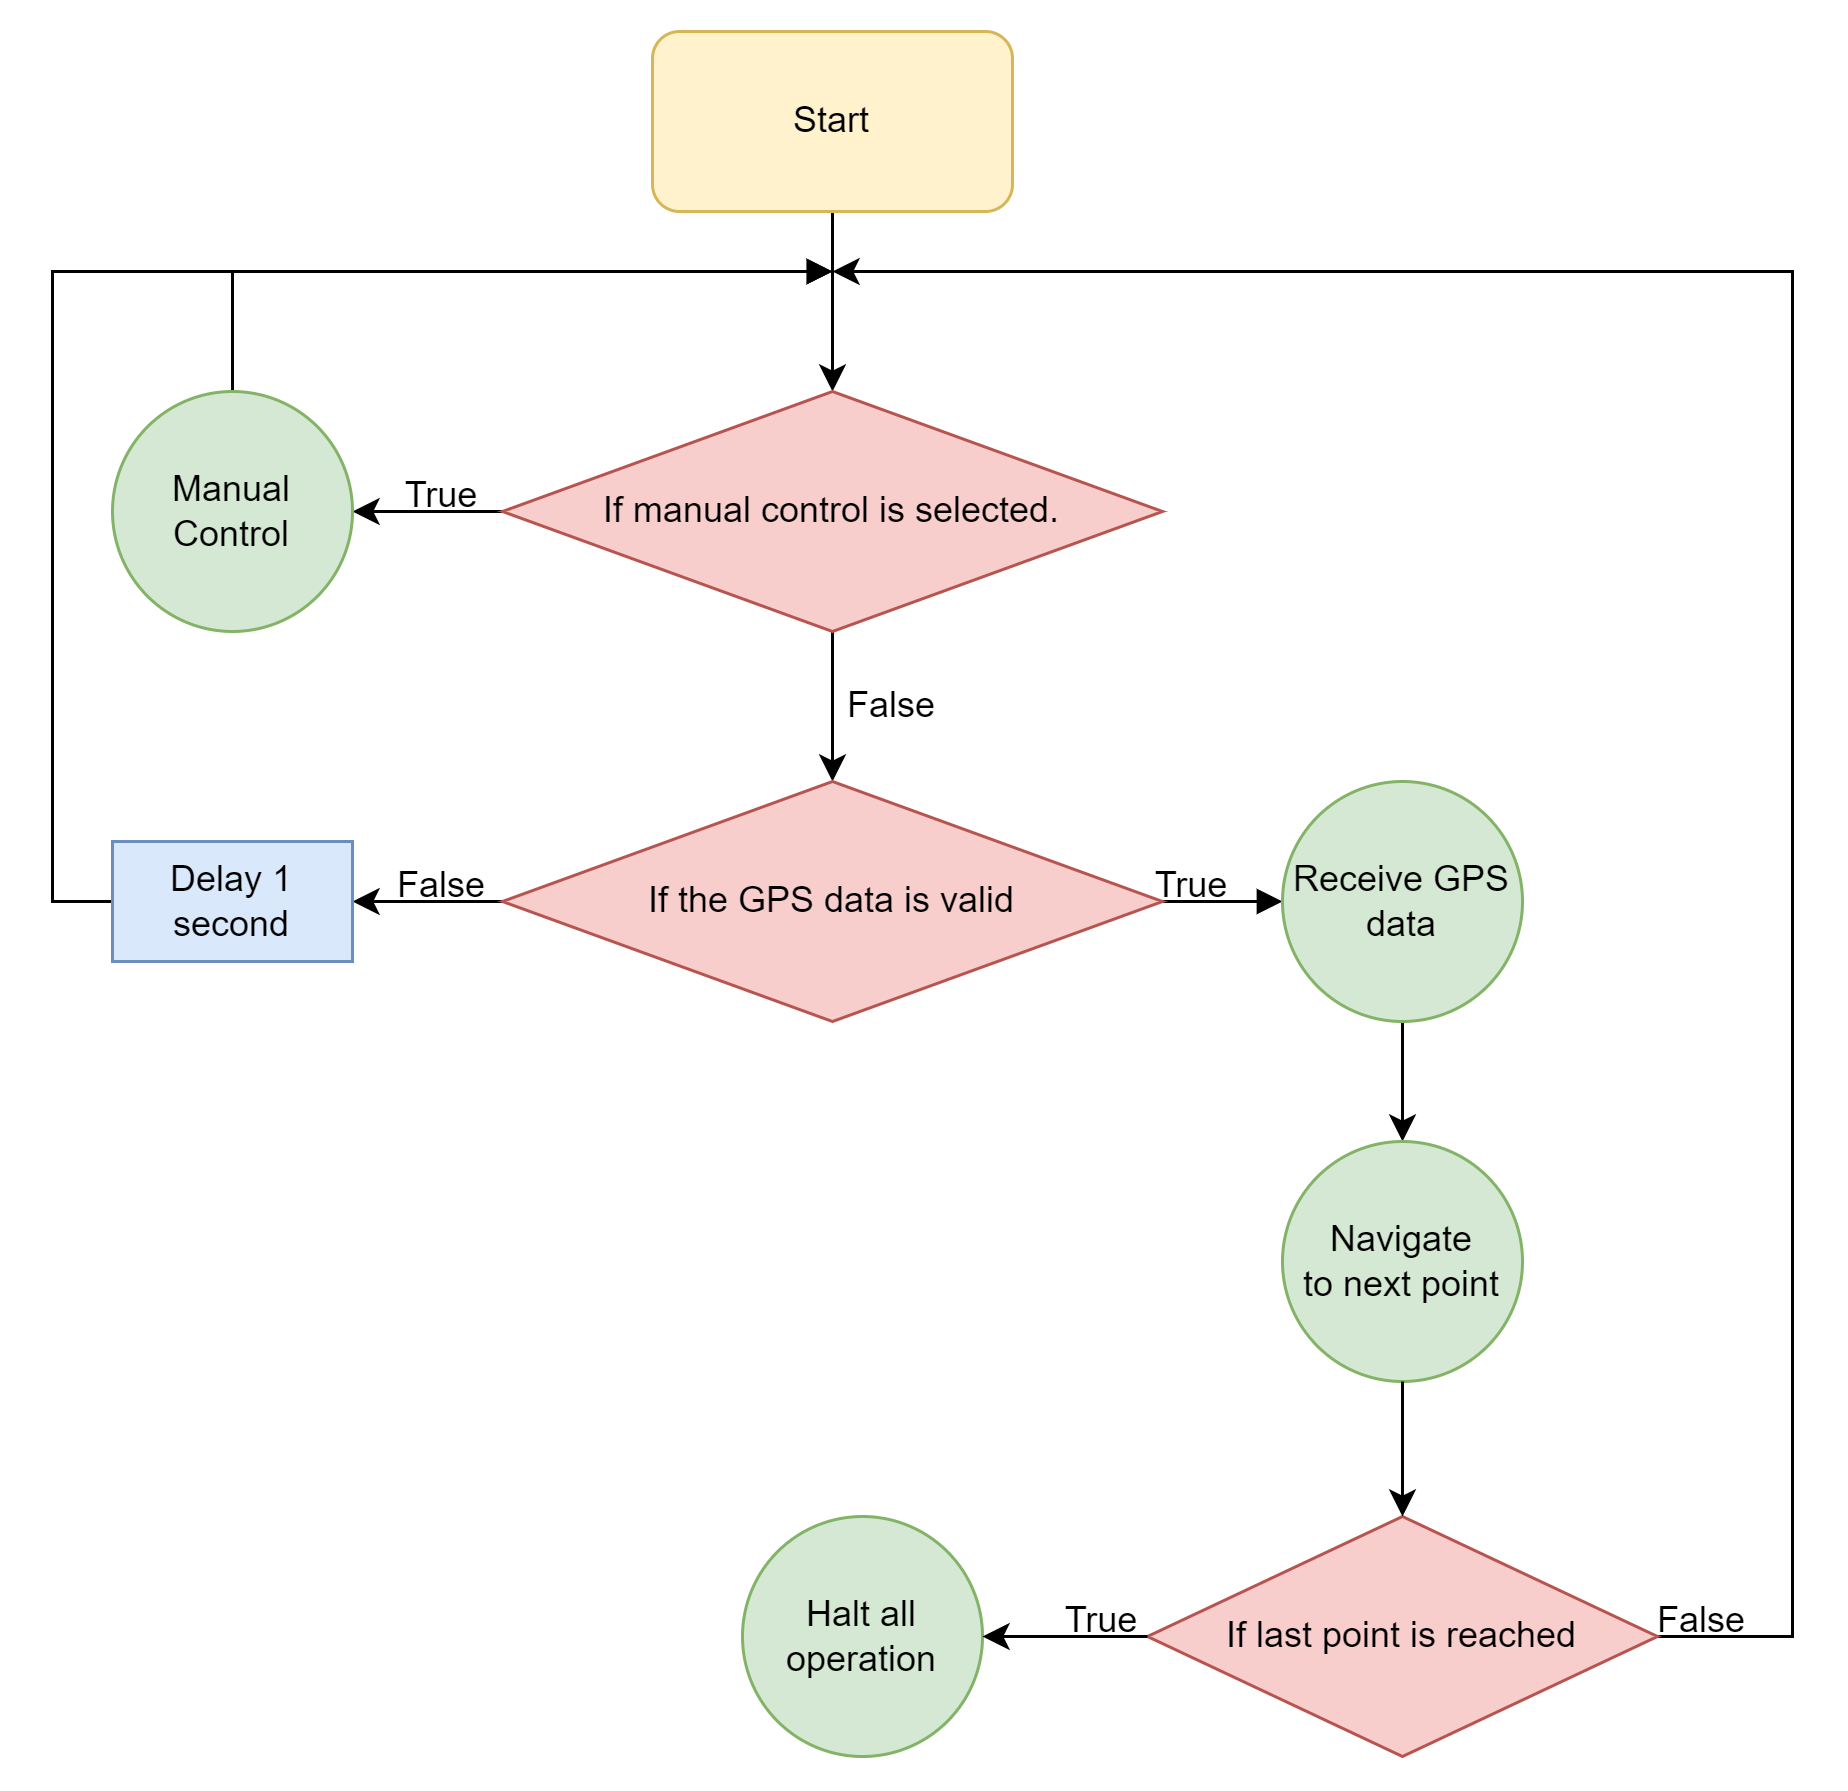
\includegraphics[width = 0.66\linewidth]{figures/statemachine.png}
			\caption{Flow diagram of the main states in the system.}
			\label{fig:3:stateMachine}
		\end{center}
	\end{figure}
		The system makes use of a state machine to switch between tasks. There are four different states in which the system can be, waiting for valid GPS, manual navigation, autonomous navigation and halt. Figure \ref{fig:3:stateMachine} shows the relationship between these states. The algorithm shown is executed in the main while loop of the microcontroller and shows one cycle. The loop starts by checking the user input. The user can select to switch between the manual and autonomous operation at any point. However, if autonomous navigation is selected and the GPS data is valid, the system will only enter manual control once the cycle has been completed. The psuedo code for this loop is shown in Algorithm \ref{alg:3:mainWhile}.
		
	
%The source code that will be discussed can be seen in Appendix \ref{Code}


\subsubsection{Manual Control}
The manual control involves receiving an input from the user and translating this to correctly power the thrusters. As seen in Algorithm \ref{alg:3:mainWhile}, the manual control involves the call of two functions: the first where most of the processing is done and the second is updating the RA register to produce the correct PWM signal. Firstly, the flow diagram of the first one, \emph{updatePWM()} is shown in Figure \ref{fig:3:updatePWM}. This shows the process to read one side's input and calculate the required duty cycle for that side's thruster. This is carried out for both sides in each cycle. As mentioned, the second function \emph{powerThruster()} simply writes the required value to RA register for the appropriate duty cycle. The psuedo for both functions are shown in the Algorthim \ref{alg:3:manualControl}.
\begin{figure}
	\begin{center}
		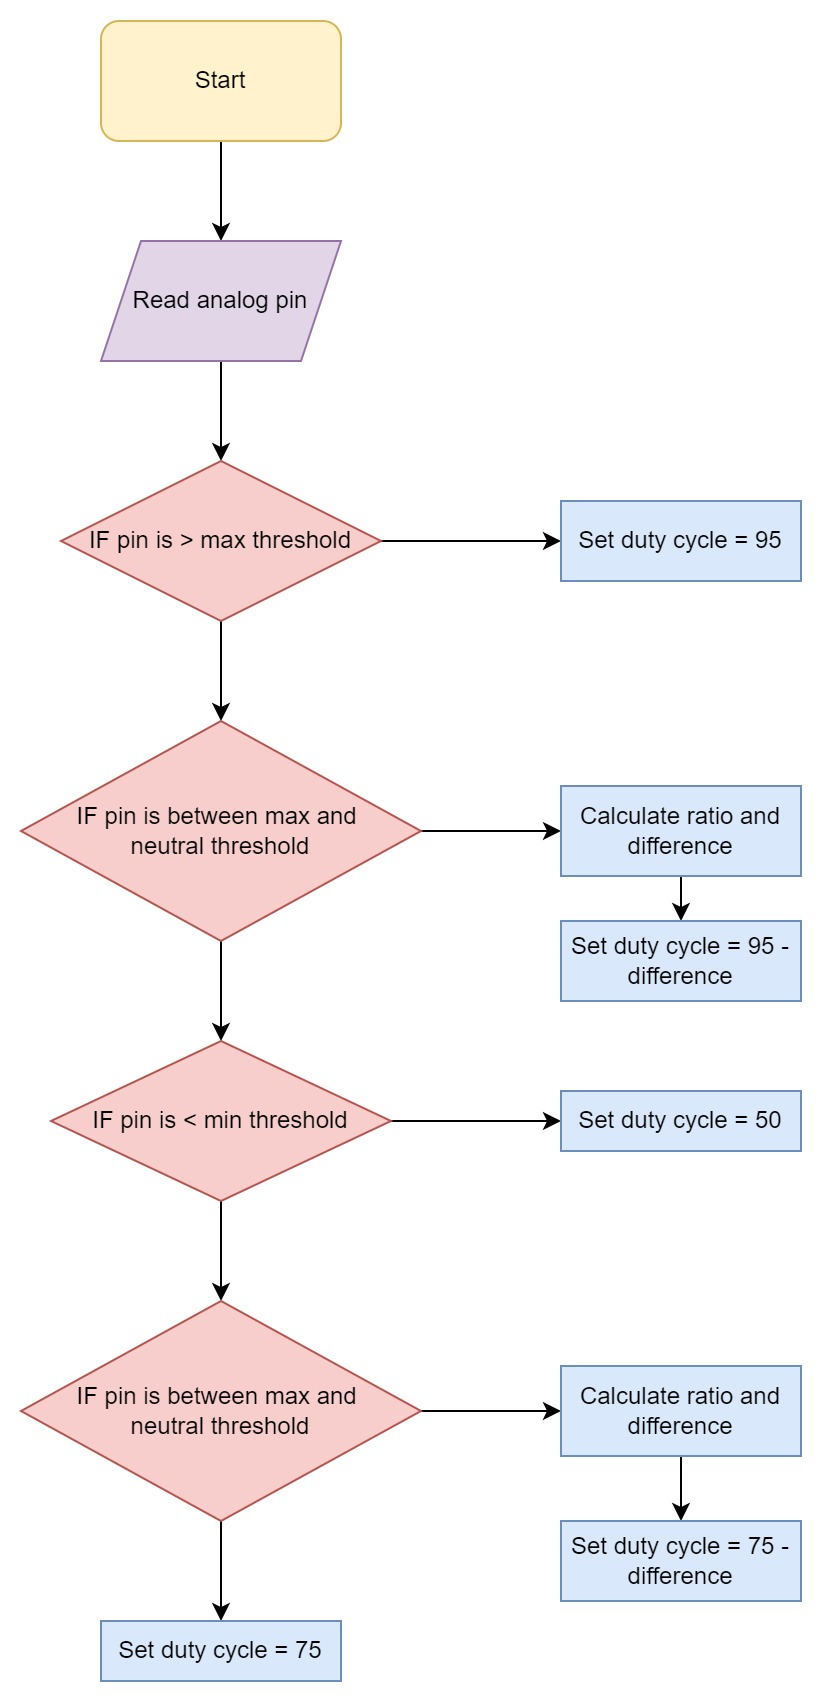
\includegraphics[width = 0.55\linewidth]{figures/UpdatePWM.jpg}
		\caption{Flow diagram of \emph{updatePWM().}}
		\label{fig:3:updatePWM}
	\end{center}
\end{figure}
\begin{algorithm}
	\caption{Pseudo code for manual control}
	\label{alg:3:manualControl}
	\begin{algorithmic}[1]
		\Procedure{updatePWM}{}
		\State $\textit{analog} \gets \textit{analogRead(analogPin)}$
		\If{$\textit{analog} > \textit{maximum threshold}$}
		\State $\textit{duty cycle} \gets 95$;
		\ElsIf{$\textit{analog}>\textit{neutral threshold}$}
		\State $\textit{analog ratio} \gets \textit{ratio forward (equ. \ref{eq:3:dutyF}) as } \textbf{float} $
		\State $\textit{difference} \gets (95 - 75) \times \textit{analog ratio as } \textbf{float}$
		\State $\textit{duty cycle} \gets 95 - \textit{difference} $
		\ElsIf{$\textit{analog} < \textit{minimum threshold} $}
		\State $\textit{duty cycle} \gets 50$;
		\ElsIf{$\textit{analog}<\textit{neutral threshold} $}
		\State $\textit{analog ratio} \gets \textit{ratio reverse (equ. \ref{eq:3:dutyR}) as }\textbf{float} $
		\State $\textit{difference} \gets (75 - 50) \times \textit{analog ratio as } \textbf{float}$
		\State $\textit{duty cycle} \gets 75 - \textit{difference}$
		\Else 
		\State $\textit{duty cycle} \gets 75$;
		\EndIf
		\EndProcedure
		\Procedure{powerThrusters}{}
		\State $\textit{RA} \gets \textit{RC} \times \textit{duty cycle\SI{}{\percent}}$;
		\EndProcedure
	\end{algorithmic}
\end{algorithm}
\subsubsection{Receiving GPS Data}
The GPS data is received with serial UART communication and is a string of characters as shown previously. To receive the correct data line, the microcontroller receives each line and then checks that it is the required line. Given the required line, the line is processed and the struct is updated with the newest data. A few small tools were written to assist in this. They are all relatively simple and so their pseudo is unnecessary but a brief description follows for context.\par
\textbf{findAllInstacesOf()}\par
This function takes an integer array, a character array to search, a character to search for and the size of the character array to search as parameters. It returns the integer array with the index positions of the character searched for.\par
\textbf{charToInteger()}\par
This function takes a character array and a start and end index as integers. It returns an integer as it would be seen as the character string. For example, the character string '4862' would be returned as 4862 as an integer.\par
\textbf{charToDecimals()}\par
This function is similar to the integer version but it returns a float with the numbers as the decimals. For example a character string of '4862' would be returned as 0.4862.\par
The overall process to receive the GPS data and populate the struct is shown in the flow diagram of Figure \ref{fig:3:recGPS}. The struct is populated by using the two arrays, containing indexes full stops and commas indexes withing the character array, to split up the character array into the necessary information. This is easily done as the string from the GPS has a standard form.
\begin{algorithm}
	\caption{Pseudo code for receiving GPS data}
	\label{alg:3:receiveGPS}
	\begin{algorithmic}[1]
		\State $\textit{msgReceived} \gets \textit{false}$
		\State $\textit{rxCnt} \gets 0$
		\While{$!\textit{msgRecieved}$}
		\While{$ \textit{rxByte} != 10$}
		\State $\textit{rxByte} \gets \textit{SerialRead()}$
		\If{$\textit{rxByte} != -1$}
		\State $\textit{rxData(rxCnt)} \gets \textit{rxByte}$
		\State $\textit{rxCnt} \gets \textit{rxCnt} + 1$ 
		\EndIf
		\EndWhile
		\If{$\textit{rxData(3) = \textit{'R' AND rxData(4)} = \textit{'M' AND rxData(5)} = \textit{'C'}}$}
		\State $\textit{call updateStructRMC(rxData, rxCnt)}$
		\State $\textit{msgReceived} \gets \textit{true}$
		\EndIf
		\State $\textit{rxCnt} \gets 0$
		\State $\textit{rxByte} \gets 0$
		\EndWhile
	\end{algorithmic}
\end{algorithm}
\begin{figure}[!hb]
	\begin{center}
		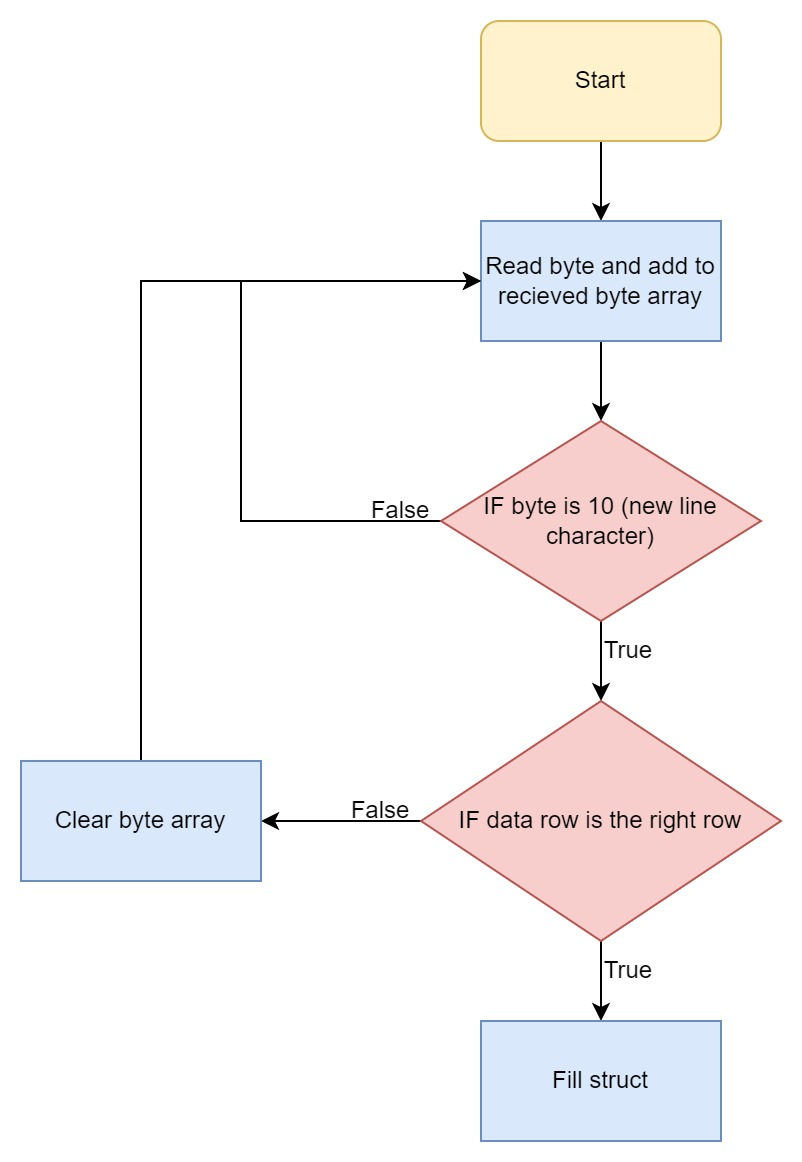
\includegraphics[width = 0.35\linewidth]{figures/receiveGPS}
		\caption{The flow diagram of receiving the GPS data.}
		\label{fig:3:recGPS}
	\end{center}
\end{figure}
\subsubsection{Autonomous Navigation}
The autonomous navigation will only begin executing when valid GPS data has been received. Therefore, there is no need to check the data when the navigation algorithm begins. The target points for the navigation are written into a text file prior to launching. The program reads these points into a struct at the start of operation to be ready for the autonomous navigation. The autonomous control calculates the distance and bearing to its destination and the error between its current bearing and its target bearing. To calculate the distance between two points that are very close together, one can use Pythagoras theorem without much error because across a small instantaneous distance the world is flat. However, due to the curvature of the earth, across much larger distances the Pythagoras theorem looses accuracy. Therefore in this project the haver-sine formula, equations \ref{equ:3:a} - \ref{equ:3:d}, is used where $\phi$ is latitude and $\lambda$ is longitude, both in radians. Furthermore, the curvature of the earth effects the bearing along the line between two points. Therefore, the bearing to target calculated in this project is the forward azimuth as this is the bearing that if followed on a straight line along the arc of the earth would lead to the final point. \cite{VanBrummelen2013}, \cite{Veness2002}, \cite{Alger1910}\par
\begin{equation}
	a = \sin{(\frac{\triangle\phi}{2})}^2 + \cos{\phi_{1}}\times\cos{\phi_{2}}\times\sin{(\frac{\triangle\lambda}{2})}^2
	\label{equ:3:a}
\end{equation}
\begin{equation}
	c = 2\times\arctan2(\sqrt{a}, \sqrt{1-a})
\end{equation}
\begin{equation}
	d = 6371000 \times c
	\label{equ:3:d}
\end{equation}
If the distance and bearing error are above a set threshold, the system will move at full power using full steering. However, once it is within the distance threshold, it will begin to slow down proportional to how close it is. The amount of throttle as a percentage is determined by a ratio of the remaining distance and the distance threshold. Furthermore, once the distance is reduced below the arrival threshold, the point is marked as 'passed' and the system will begin navigating to the next point or halt operation if there are no more points. Similarly for the steering, the amount of steering as a percentage is a ratio of the bearing error and the steering threshold. Finally, the direction to steer in is determined using an equation that accounts for the \SI{360}{\degree}/\SI{0}{\degree} turnover point. If the target bearing is anywhere within \SI{180}{\degree} to the right of the current bearing, it will turn right and visa versa. This logic and pseudo code can be seen in the flow diagram of Figure \ref{fig:3:autoNav} and Algorithm \ref{alg:3:autoNav}. In the pseudo code only the procedure for \emph{steerLeft()} is shown as the procedure for \emph{steerRight()} follows the exact same logic but with the thruster sides inverted. 

\begin{figure}
	\begin{center}
		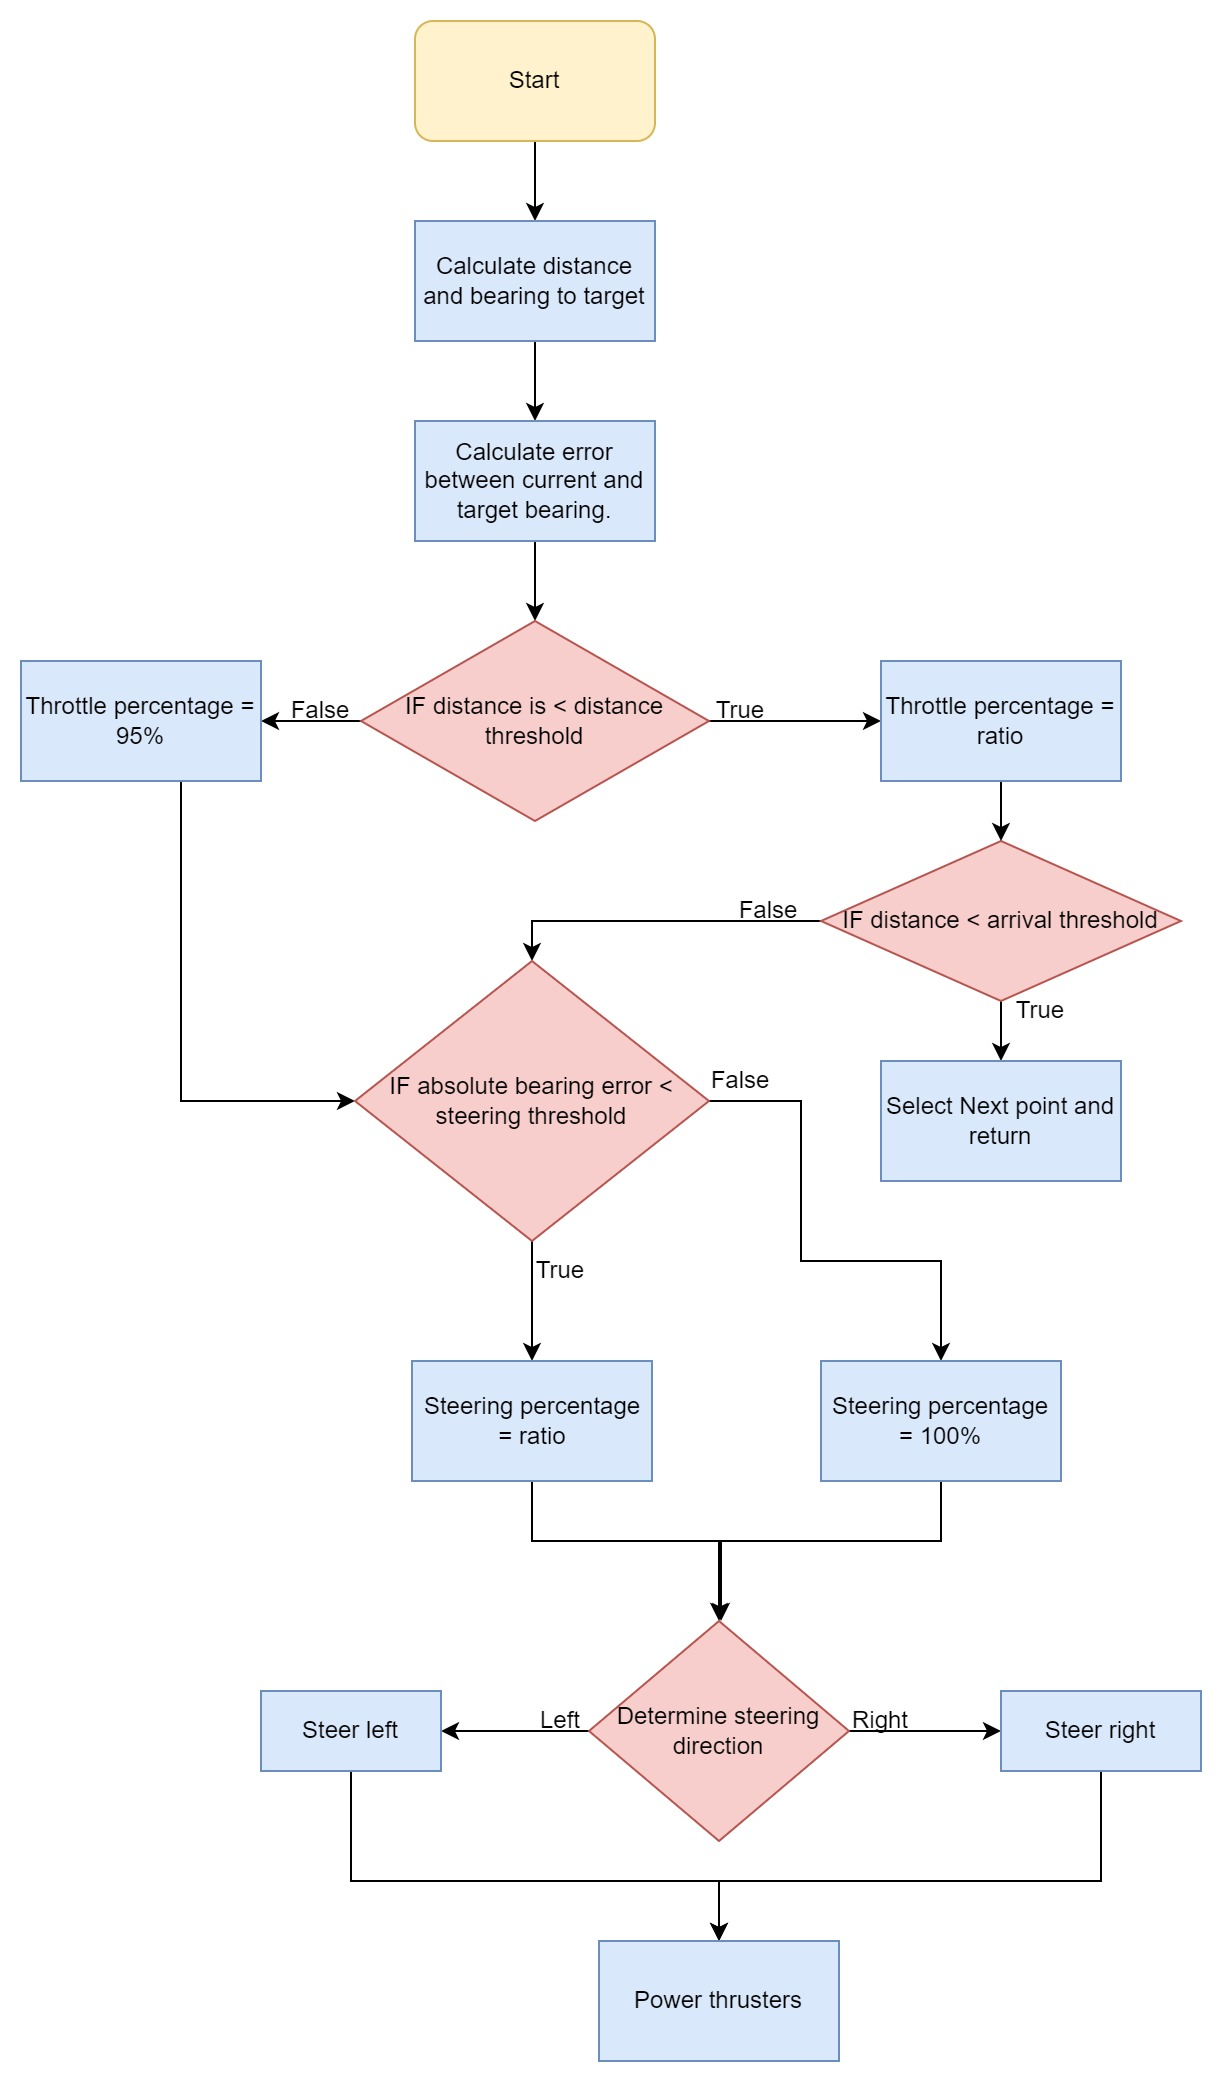
\includegraphics[width=0.7\linewidth]{figures/autoNav.jpg}
		\caption{Flow diagram of the autonomous navigation}
		\label{fig:3:autoNav}
	\end{center}
\end{figure}
\begin{algorithm}
	\caption{Pseudo code for the autonomous navigation}
	\label{alg:3:autoNav}
	\begin{algorithmic}[1]
		\Require{Read the target GPS points from SD card.}
		\Procedure{navigate()}{}
		\State $\textit{Calculate distance to target}$
		\State $\textit{Calculate bearing to target}$
		\State $\textit{Calculate the error between current and target bearing}$
		\If{$\textit{distance} < \textit{distance threshold}$}
		\State $\textit{throttle percentage} \gets \frac{\textit{distance}}{2 \times \textit{distance threshold}} $
		\If{$\textit{distance} < \textit{arrival threshold}$}
		\State $\textit{call NextPoint()}$
		\State $\textbf{return}$
		\EndIf
		\Else 
		\State $\textit{throttle percentage} \gets 95$
		\EndIf
		\If{$\textit{abs(bearing error)} < \textit{steering threshold}$}
		\State $\textit{steering percentage} \gets \frac{\textit{abs(bearing error)}}{\textit{steering threshold}}$
		\Else
		\State $\textit{steering percentage} \gets 100$
		\EndIf
		\State $\textit{maxBearing} \gets \textit{max(bearing error, target bearing)}$
		\State $\textit{minBearing} \gets \textit{min(bearing error, target bearing)}$
		\If{$(\textit{maxBearing = target bearing}) \textit{XOR} (\textit{maxBearing} - \textit{minBearing}) >180 )$}
		\State $\textit{call steerLeft()}$
		\Else
		\State $\textit{call steerRight()}$
		\EndIf
		\State $\textit{call powerThrusters()}$
		\EndProcedure
		\Procedure{NextPoint()}{}
		\State $\textit{points(targetIndex).passed} \gets \textit{true}$
		\State $\textit{targetIndex} \gets \textit{targetIndex} + 1$
		\If{$\textit{points.targetIndex does not exists}$}
		\State $\textit{state} \gets \textit{Halt navigation}$
		\EndIf
		\EndProcedure
		\Procedure{steerLeft()}{}
		\State $\textit{throttle difference} = 2 \times \textit{throttle percentage}$
		\State $\textit{rightSide.duty Cycle} \gets 75 + (25 \times (\textit{throttle percentage}\SI{}{\percent}))$
		\State $\textit{leftSide.duty Cycle} \gets \textit{rightSide.duty Cycle} - (25 \times ((\textit{throttle difference} \times (\textit{steering percentage}\SI{}{\percent}))/100))$
		\EndProcedure
	\end{algorithmic}
\end{algorithm}